%______________________________________________________________________
\clearpage
\section*{\citet{2018_Lucena}}
%______________________________________________________________________

\subsection*{Authors}
The authors of the paper can be viewed in table \ref{tab:2018_Lucena_Authors}.
\begin{longtable}{ |P{3cm}|P{4cm}|P{5cm}| }
	\caption{Authors} \label{tab:2018_Lucena_Authors} \\
	\hline
 	\cellcolor{Gray}Name & \cellcolor{Gray}Location & \cellcolor{Gray}Institution \\ [0.5ex] 
 	\hline\hline
 	\endhead
 	Percival Lucena & \multirow{2}{4cm}{\centering Brazil}  & \multirow{2}{5cm}{\centering IBM Research\urlfootnote{https://researcher.watson.ibm.com/researcher/view_group_pubs.php?grp=5113}} \\
	\cline{1-1}
	 Alecio P. D. Binotto &   &  \\
	 \hline
	 Fernanda da Silva Momo & Porto Alegre, Brazil  &  Federal University of Rio Grande do Sul (UFRGS) \nomenclature[U]{UFRGS}{Federal University of Rio Grande do Sul}\\
	 \hline
	 Henry Kim & Toronto, Canada  & York University\\
	 \hline
\end{longtable}

%______________________________________________________________________

\subsection*{Contribution}
The contribution of \citet{2018_Lucena} is a grain quality assurance tracking system.
Their work is not available open source.

%______________________________________________________________________

\subsection*{Reason/Problems}
The brazilian \quoteit{Grain Exports Business Network (GEBN)}\nomenclature[O]{GEBN}{Grain Exports Business Network} is composed of the following actors:
\begin{enumerate}[label={\arabic*)},font={\color{red!50!black}\bfseries},noitemsep]
	\item \textbf{Grain Producer}
	\item \textbf{Rural Credit Bank agent}
	\item \textbf{Private warehouse agent}
	\item \textbf{Trading company agent}
	\item \textbf{Food processing company}
\end{enumerate}
\clearpage
\begin{longtable}{ |P{3cm}|P{4cm}|P{5cm}| }
	\caption{Authors} \label{tab:2018_Lucena_Authors} \\
	\hline
 	\cellcolor{Gray}Actor & \cellcolor{Gray}Concern & \cellcolor{Gray}Reason \\ [0.5ex] 
 	\hline\hline
 	\endhead
	\multirow{3}{3cm}{\centering Grain Producer} & Correct management of grain ingest and classification & Receive a fair payment \\
	\cline{2-3}
	 & \multirow{2}{4cm}{\centering Proper ingest receipt} & Acquire a credit on Rural Credit Banks\\
	 \cline{3-3}
	 & & Agree on a production insurance \\
	 \hline
	 Rural Credit Bank agent & \multirow{2}{4cm}{\centering Accurate data from producers} & Lower credit giving risks\\
	 \cline{3-3}
	 & & Offer reduced interest credit rates for credit operations\\
	 \hline
	 Private Warehouse agent & Precise grain classification data & Sell the grains to various actors \\
	 \hline
	 Trading Company agent & Purchase of large amounts of grains with the right quality from several warehouses & Achieve an export request \\
	 \hline
	 Food processing company & Acquisition of special selected grains that have specific characteristics (e.g.\ high protein) & \xmark \\
	 \hline
\end{longtable}


\begin{figure}[!ht]
    \centering
    \label{fig:2018_Lucena_Implementation_Business}
    \caption{Business Network}
    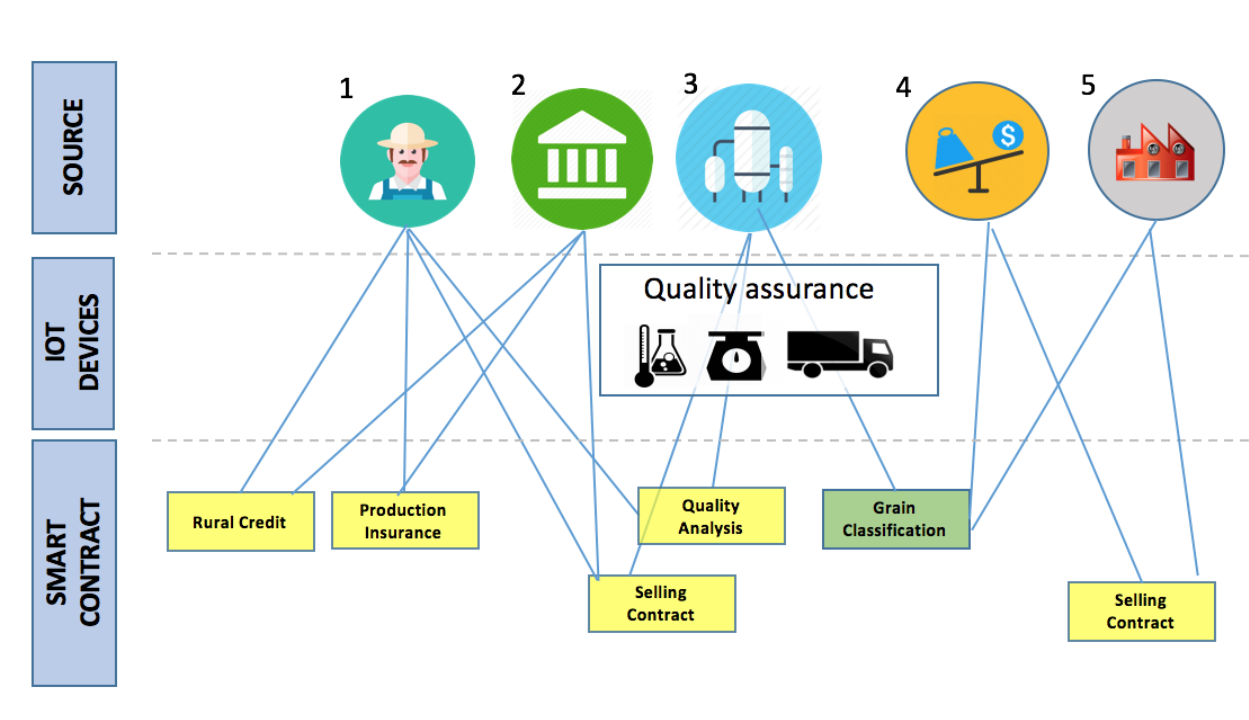
\includegraphics[width=0.8\textwidth]{2018_Lucena_1.png}
\end{figure}

%______________________________________________________________________

\subsection*{Implementation Process}

\begin{figure}[!ht]
    \centering
    \label{fig:2018_Lucena_Implementation_Architecture}
    \caption{Architecture}
    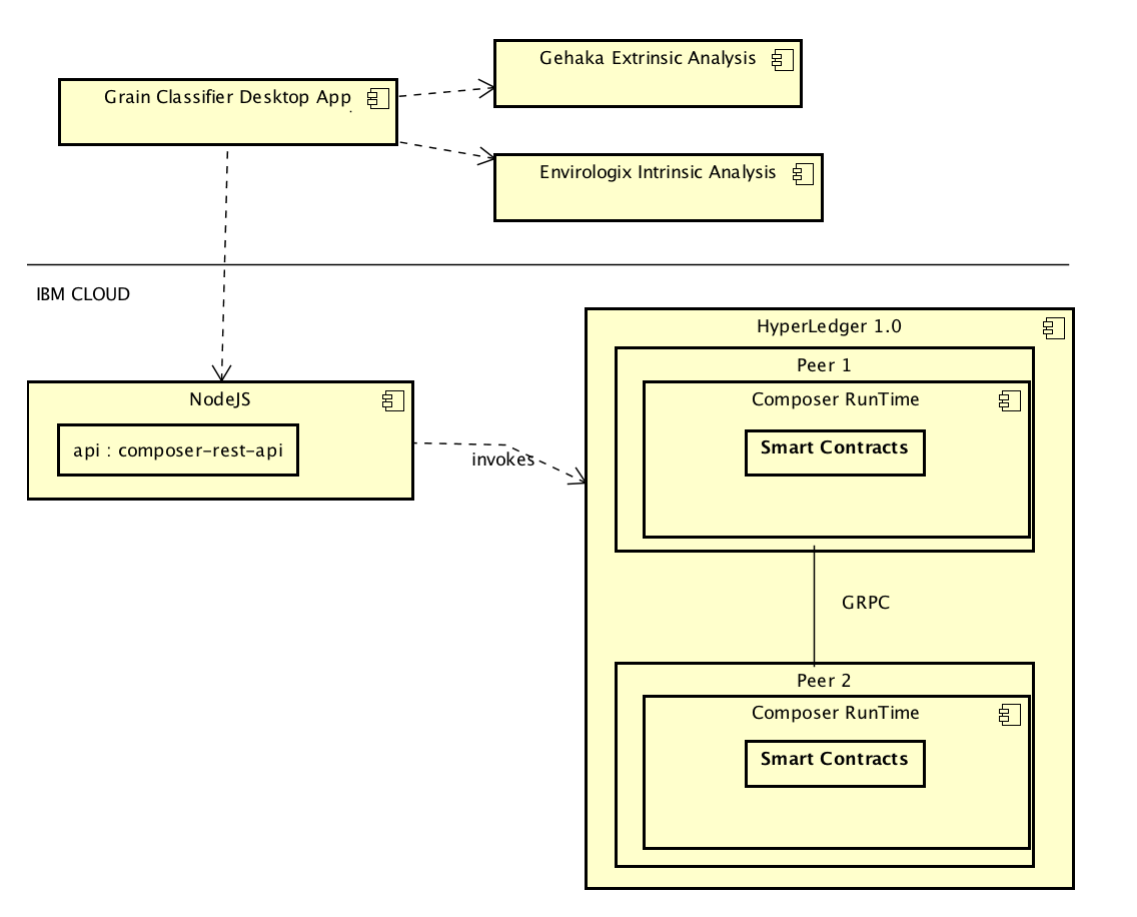
\includegraphics[width=0.8\textwidth]{2018_Lucena_2.png}
\end{figure}
%______________________________________________________________________

\subsection*{Conclusion}

